\documentclass[a4paper,11pt]{scrartcl}

\usepackage[shortlabels]{enumitem}
\usepackage{csquotes}
\usepackage[utf8]{inputenc}
\usepackage[T1]{fontenc}
\usepackage[top=1.3in, bottom=1in, left=1.0in, right=0.6in]{geometry}
\usepackage{fancyhdr}
\usepackage[hidelinks]{hyperref}
\usepackage{minted}
\usepackage{tikz}
\usepackage{array}
\usepackage{amsmath}
\usepackage{setspace}
\usepackage{lastpage}

\author{Alexander Timmermann, Jannis Krämer}
\title{GSS-Übungsblatt 2}
\date{}

\pagestyle{fancy}
\fancyhf{}
\fancyhead[C]{Alexander Timmermann, Jannis Krämer}
\fancyhead[L]{Blatt 2}
\fancyhead[R]{Seite~\thepage\ von \pageref{LastPage}}

\usemintedstyle{tango}
\usetikzlibrary{arrows}

\begin{document}

\maketitle
\thispagestyle{empty}

\doublespace

\section{Grundlagen von Betriebssystemen}

\begin{enumerate}[\bf a)]
    \item
        \begin{enumerate}[1.]
            \item Verwaltung von Betriebsmitteln, d.h. OS als
                  \textbf{``Betriebsmittelverwalter''.} Das OS übernimmt die
                  Ermittlung, Zuteilung und Verwaltung der nötigen
                  Betriebsmittel (Platz im Speicher, CPU-Zeit,…)
            \item Abstraktion der Hardware, d.h. OS als
                  \textbf{``virtuelle Maschine''.} Das OS macht durch die
                  Abstraktion die Hardware für den Endnutzer bedienbar und
                  bietet ein (im besten Falle) universelles Interface für
                  Programme.
        \end{enumerate}
    \item
        \begin{enumerate}[1.]
            \item
                \begin{enumerate}[$\star$]
                    \item Zuordnung von Betriebsmitteln an Prozesse, d.h. RAM,
                          CPU-Zeit,…
                    \item Behandlung von Ressourcen-Konflikten und -Engpässen,
                          insbesondere z.B. race conditions oder Programme in
                          einer Endlosschleife.
                \end{enumerate}
            \item
                \begin{enumerate}[$\star$]
                    \item Rechnerarchitektur vor dem Nutzer verbergen, da sie in
                          den meisten Fällen irrelevant ist.
                    \item Hardwareunabhängigkeit durch Abstraktion herstellen
                \end{enumerate}
        \end{enumerate}
\end{enumerate}

\section{Prozesse und Threads}

\begin{enumerate}[\bf a)]
    \item
        \begin{description}
            \item[Programm:] Ein Programm ist eine vordefinierte Anzahl von
                             Anweisungen an den Computer bzw. das Betriebssystem
                             als Abstraktionslayer. Programme werden meist in
                             höheren Programmiersprachen geschrieben und dann in
                             für den Computer verständlichen Bytecode übersetzt.

            \item[Prozess:]  Ein Programm wird in einem sog. Prozess ausgeführt,
                             dem vom Betriebssystem ein eigener Bereich im Speicher
                             des Computers zugewiesen wird.

            \item[Thread:]   Ein Thread ist eine Art ``Miniprozess'', der einem
                             Prozess zugeordnet ist und sich mit den anderen
                             Threads eines Prozesses den gleichen Bereich im
                             Arbeitsspeicher teilt.
        \end{description}

    \item[\bf d)]
		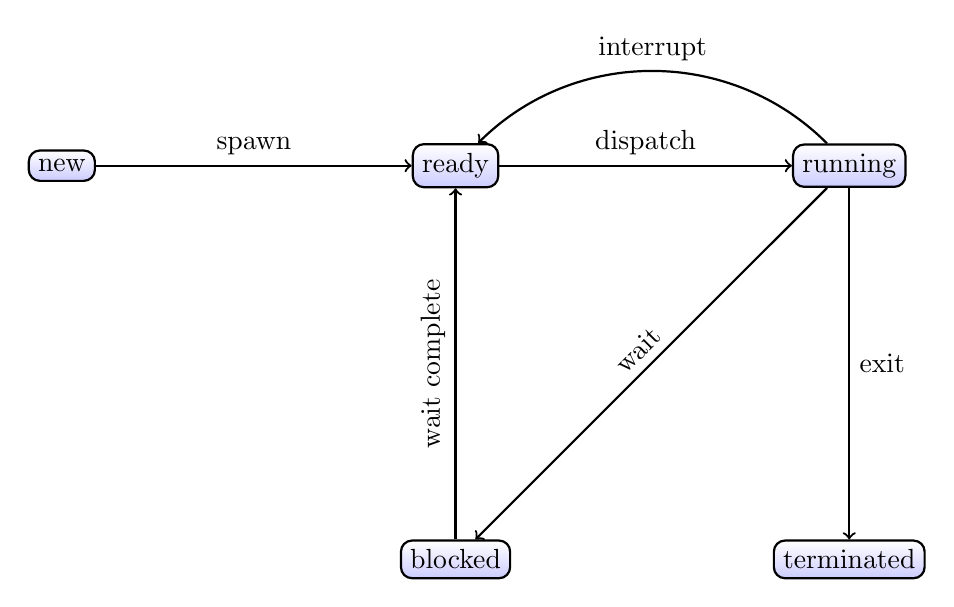
\begin{tikzpicture}[baseline=(current bounding box.north),node distance=5cm,->,thick,main/.style = {shape=rectangle, rounded corners,draw, align=center,top color=white, bottom color=blue!20}]
			\node (new) [main] {new};
			\node (ready) [main,right of=new] {ready};
            \node (running) [main,right of=ready] {running};
            \node (blocked) [main,below of=ready] {blocked};
            \node (terminated) [main,below of=running] {terminated};

            \path (new) edge node[above] {spawn} (ready);
            \path (ready) edge node[above] {dispatch} (running);
            \path (blocked) edge[sloped] node[above] {wait complete} (ready);
            \path (running) edge[sloped] node[above] {wait} (blocked);
            \path (running) edge node[right] {exit} (terminated);
            \path (running) edge[bend right=45] node[above] {interrupt} (ready);
		\end{tikzpicture}~\\~\\

        \begin{description}
            \item[ready:] Ausführung möglich, jedoch momentan angehalten
            \item[running:] Benutzung der CPU zur Berechnung
            \item[blocked:] Ausführung hält und wartet auf externen Input
            \item[spawn:] Prozess wird erstellt und wechselt in Zustand \textit{ready}
            \item[dispatch:] Dispatcher weist Aufgabe zu, die ausgeführt wird
            \item[interrupt:] laufender Prozess wird vom Betriebssystem unterbrochen
            \item[wait:] laufender Prozess wechselt in \textit{blocked}-Zustand, d.h. wartet auf externen Input
            \item[wait complete:] Input ist erfolgt, Prozess bereit zur weiteren Ausführung
            \item[exit:] Der Prozess terminiert
        \end{description}
\end{enumerate}

\section{n-Adressmaschine}

\begin{enumerate}[\bf a)]
    \item
        \textbf{2-Adressmaschine}, 8 Befehle, 13 Lese- und 8 Schreiboperationen\\
        \begin{tabular}{>{\ttfamily}p{1cm} >{\ttfamily}p{1cm} >{\ttfamily}p{2cm} | >{\ttfamily}p{5cm}}
            MOVE & >$\mathtt a_1$< & >$\mathtt H_1$< & $H_1 := a_1$ \\
            ADD  & >$\mathtt a_2$< & >$\mathtt H_1$< & $H_1 := a_1 + a_2$\\
            DIV  & >$\mathtt H_1$< & >$\mathtt a_3$< & $H_1 := \frac{a_1 + a_2}{a_3}$\\
            MOVE & >$\mathtt b_2$< & >$\mathtt H_2$< & $H_2 := b_2$\\
            SUB  & >$\mathtt b_1$< & >$\mathtt H_2$< & $H_2 := b_1 - H_2 = b_1 - b_2$\\
            DIV  & >$\mathtt H_2$< & >$\mathtt b_3$< & $H_2 := \frac{b_1 - b_2}{b_3}$\\
            MOVE & >$\mathtt H_1$< & >R<             & $R := H_1 = \frac{a_1 + a_2}{a_3}$\\
            ADD  & >$\mathtt H_2$< & >R<             & $R := R + H_2 = \frac{a_1 + a_2}{a_3} + \frac{b_1 - b_2}{b_3}$
        \end{tabular}

    \item
        \textbf{1-Adressmaschine}, 8 Befehle, 13 Lese- und 8 Schreiboperationen\\
        \begin{tabular}{>{\ttfamily}p{1cm} >{\ttfamily}p{3.46cm} | >{\ttfamily}p{5cm}}
            LOAD & >$\mathtt b_1$< & $AC := b_1$\\
            SUB  & >$\mathtt b_2$< & $AC := b_1 - b_2$\\
            DIV  & >$\mathtt b_3$< & $AC := \frac{b_1-b_2}{b_3}$\\
            SAVE & >$\mathtt H_1$< & $H_1 := AC$\\
            LOAD & >$\mathtt a_1$< & $AC := a_1$\\
            ADD  & >$\mathtt a_2$< & $AC := a_1 + a_2$\\
            DIV  & >$\mathtt a_3$< & $AC := \frac{a_1 + a_2}{a_3}$\\
            ADD  & >$\mathtt H_1$< & $AC := \frac{a_1 + a_2}{a_3} + \frac{b_1-b_2}{b_3}$\\
            SAVE & >R<
        \end{tabular}

    \pagebreak

    \item
        \textbf{Stack-Rechner}, 12 Befehle, 6 Leseoperationen\\
        \begin{tabular}{>{\ttfamily}p{1cm} >{\ttfamily}p{3.46cm} | >{\ttfamily}p{5cm}}
            PUSH & >$\mathtt a_1$< & \fbox{$a_1$}\\
            PUSH & >$\mathtt a_2$< & \fbox{$a_1$} \fbox{$a_2$}\\
            ADD  &                 & \fbox{$a_1 + a_2$}\\
            PUSH & >$\mathtt a_3$< & \fbox{$a_1 + a_2$} \fbox{$a_3$}\\
            DIV  &                 & \fbox{$\frac{a_1 + a_2}{a_3}$}\\
            PUSH & >$\mathtt b_1$< & \fbox{$\frac{a_1 + a_2}{a_3}$} \fbox{$b_1$}\\
            PUSH & >$\mathtt b_2$< & \fbox{$\frac{a_1 + a_2}{a_3}$} \fbox{$b_1$} \fbox{$b_2$}\\
            SUB  &                 & \fbox{$\frac{a_1 + a_2}{a_3}$} \fbox{$b_1 - b_2$}\\
            PUSH & >$\mathtt b_3$< & \fbox{$\frac{a_1 + a_2}{a_3}$} \fbox{$b_1 - b_2$} \fbox{$b_3$}\\
            DIV  &                 & \fbox{$\frac{a_1 + a_2}{a_3}$} \fbox{$\frac{b_1 - b_2}{b_3}$}\\
            ADD  &                 & \fbox{$\frac{a_1 + a_2}{a_3} + \frac{b_1 - b_2}{b_3}$}\\
            POP  & >$\mathtt R$<
        \end{tabular}

\end{enumerate}

\end{document}
